\section{Confidential Services}
In this section I present two Confidential Cloud Services. The first one is the Confidential Consortium Framework (CCF)~\cite{Howard} and the second one is Nimble~\cite{Nimble}. They both provide a structure to guarantee the CIA properties, but have some differences in their design, especially when it comes to rollback attacks. Nimble is specialized in detecting rollback attacks while CCF is a whole framework that can also be used for multiparty applications.

\subsection{CCF in a nutshell}
The basic idea of CCF is that an untrusted host exists and one or more untrusted users can access the application via different replicated nodes that are responsible for the remaining communication. Providers only need to implement the application logic and make sure to have all necessary endpoints, so that CCF can handle these. Users then only have to access the specific endpoints to use the application. As CCF is especially implemented for multiparty applications, it has a multiparty governance to guarantee the confidentiality and integrity. Details are elsewhere, but it consists of a constitution with proposals and ballots that can be individually customized by the application. In Figure~\ref{ccf} the structure of one node is described. The application logic gets the data from the Key-value-store which gets the data from the Consensus which is an explicit layer that is responsible for coordinating CCF in tasks like replicating nodes or making elections decisions.
  The Transaction Handler stores every signature transaction in an append-only ledger that is redundantly stored by the one of the nodes that is called primary in every other node and the persistent storage. Performing the application logic inside a TEE is fundamental for the confidentiality and the integrity, replicating the transactions is necessary for the high availability.\\ %The ledger is stored outside the TEE what leads to problems that are discussed in~\ref{challenges:ccf}.
While the primary is responsible for handling the users' requests, the remaining nodes are there as a backup. Users can get connected to any node and the specific request is either being forwarded to the primary or handled by the node itself, which is only possible for read-only requests. Every other request has to be forwarded to the primary that executes it.\\
 If a node in use fails, the user can be connected to another node, but if the primary fails there is a primary election that selects a new primary with certain voting criteria. Note that this paper focuses mostly on the functions and challenges of CCF and therefore does not go into detail about how the election works. \\
 User requests are handled as transactions, that have a unique transaction ID. The primary also periodically sends signature transactions that verify all previous transactions as committed. To commit these signature transactions, the primary has to copy it onto at least $\lceil\frac{n-1}{2}\rceil$ nodes, where $n$ is the number of all nodes, to commit the it.\\
  Signature transactions can also confirm that there were no malicious changes to the code and thus guarantee the integrity of CCF via merkle proof~\cite{merkle}. Transactions are provided via a merkle tree, where each transaction is represented as a hash value. Every two nodes in the merkle tree are combined with a hash function to a new node. On top of the merkle tree is the merkle root, which is the value that is used for the signature transaction. This process is also shown in Figure~\ref{merkle}.\\
  
  \begin{figure}[t]
	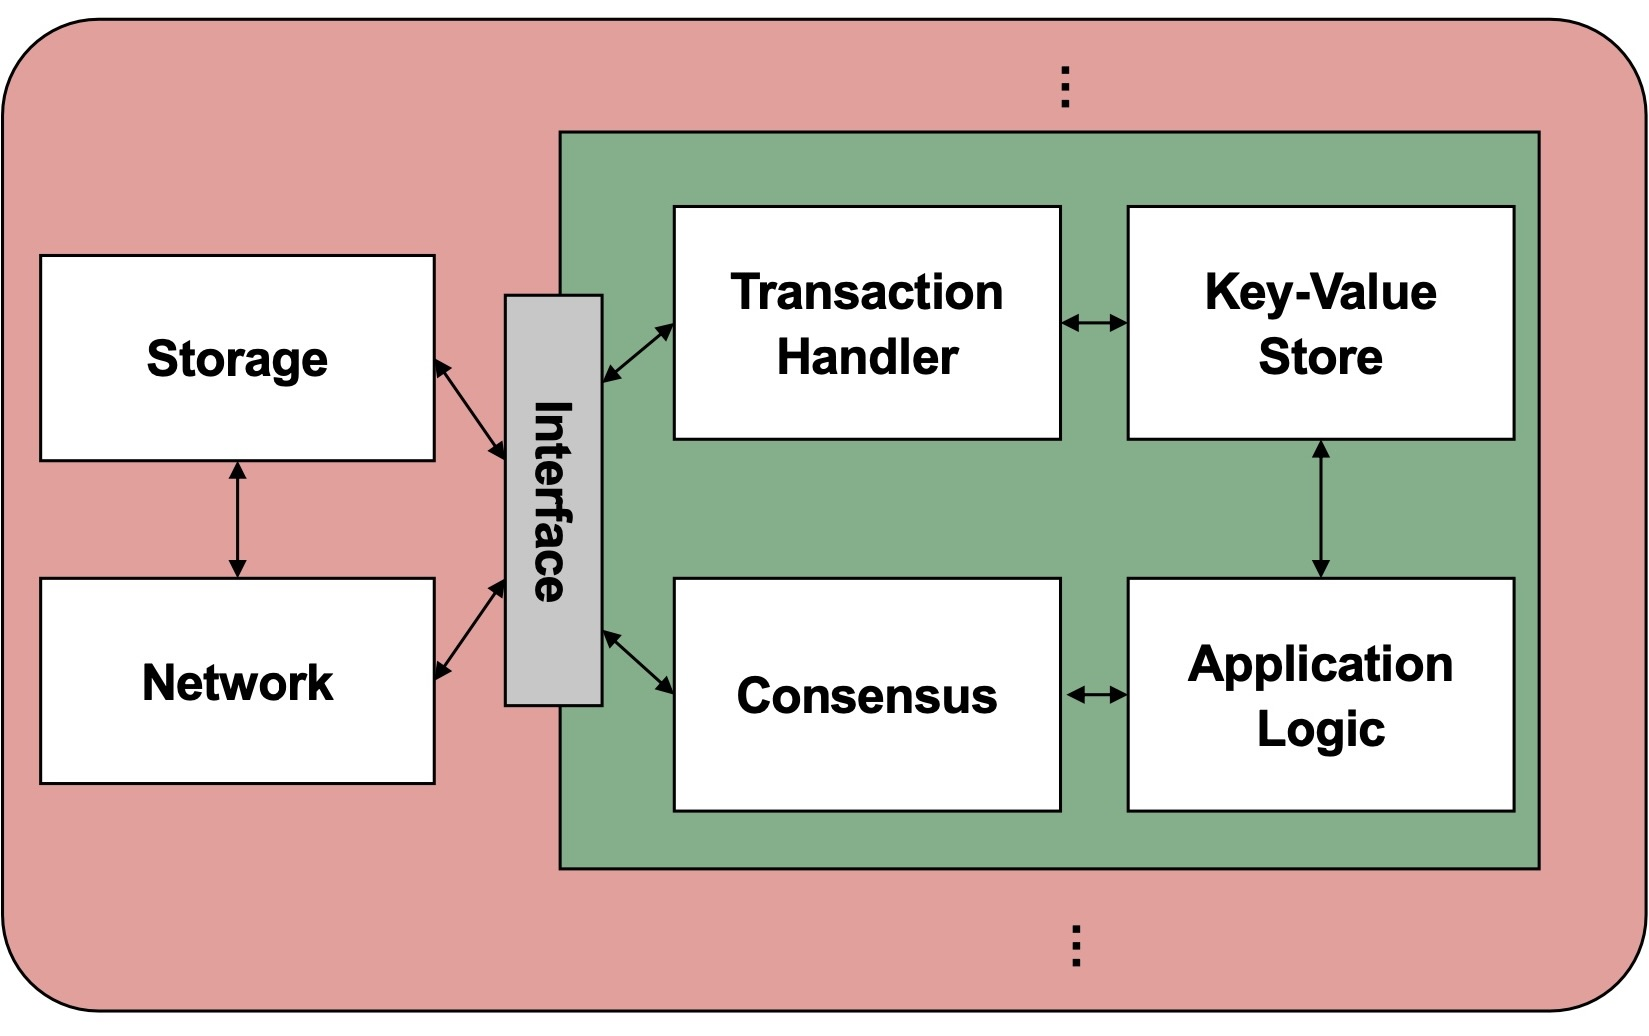
\includegraphics[scale=0.14]{pictures/ccf}
	\caption{The untrusted host consists of the network and the storage and multiple TEEs (in this figure only one TEE is shown as the inner green box) that can communicate with the outside via a interface. Inside of each TEE that refers to one node in CCF there is the Transaction Handler, the simple Key-Value Store, the individual Application Logic and the Consensus.}
	\label{ccf}
\end{figure}
  
  \subsubsection*{Reconfiguration.}
  Reconfiguration is the procedure when a node fails and is replaced by a new one. This is an important feature to guarantee the high availability.\\
CCF therefore allows to add new or delete old nodes. Reconfiguration is implemented as a transaction. For Reconfiguration a node must request an election and win it. The election is done by a majority quorum. Since a reconfiguration is handled as a transaction, it can also be rolled back. In contrast to Nimble CCF does not detect or protect such an attack on a reconfiguration.\\%TODO: write more
In a disaster scenario, a majority of nodes failed and the system has to handle this.CCF has a disaster recovery protocol, in which the service is started with an older state. Therefore it cannot be guaranteed to be complete. If not all transactions are stored at the ledger before the disaster, it cannot be restored. \\
  Although the integrity of CCF is protected by these signature transactions, the integrity can be violated via rollback attacks. While CCF avoids whole nodes to be rolled back with the help of reconfiguration the ledger is stored outside the TEE and can be attacked this way. This is a huge risk for applications with high safety requirements, because whole transactions could be undone. This also leads to certain problems in the reconfiguration that are also discussed later. Therefore I present another confidential cloud service, called Nimble, that has a rollback detection and protection mechanism and also supports reconfiguration to realize better integrity guarantees.
   %TODO: focus more on the encryption in previous part
 

\begin{figure}[t]
	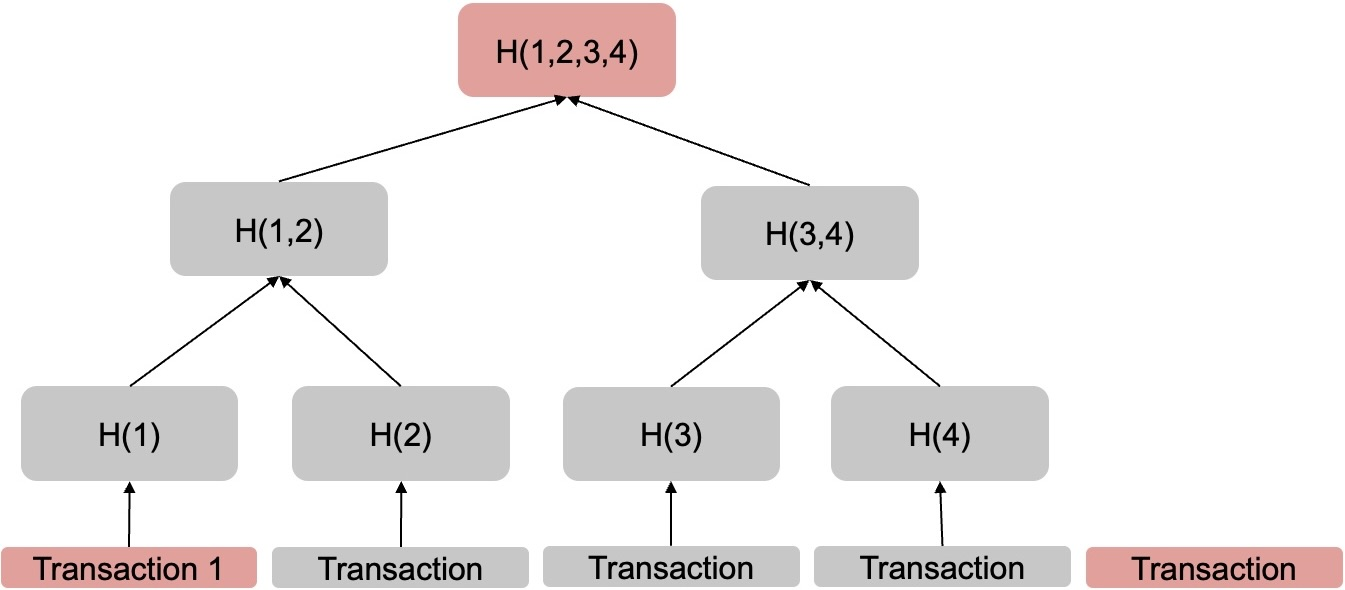
\includegraphics[scale=0.18]{pictures/merkle_tree}
	\caption{CCF's merkle tree - For every transaction a hash value is computed. Then building a new hash value from the two previous values is repeated until there is only one value left. This is called the merkle root. It is used for the signature transactions that are shown in red signed by the primary.}
	\label{merkle}
\end{figure}



\subsection{Nimble in a nutshell?}
Nimble is a state machine replication protocol that also tries to ensure the requirement of the CIA triad, but has the focus of preventing rollback attacks. The correctness of Nimble can be proofen, details about this can be found in~\cite{Nimble}.\\
Nimble has three important goals, (1) ensure linearizability, (2) having a small Trusted Computing Base (TCB) and (3) guaranteeing liveness of the cloud service. For the aim to reduce the TCB they try to use as much of the existing services the cloud provider already uses as possible. The existing cloud storage service Nimble reuses only has the requirement to be crash fault-tolerant. Therefore they use state machine replication and differ between two main properties that come with this.\\
	\textbf{\textit{Safety}} means that it must be ensured that every data that can be accessed must be the current data and must not be an older version. This property is enabled via TEEs. In the CIA triad this would be Confidentiality and Integrity.\\
	\textbf{\textit{Liveness}} is the High Availability property of the CIA triad. This has not to be ensured via a TEE, because liveness can be easily taken away even in an TEE, and can be handled outside what simultaneously makes the TCB smaller.
	To guarantee liveness Nimble stores the data redundantly via state machine replication. To guarantee safety the state of each replicated node is apended to a ledger which is stored as a hash chain in an existing storage provider. Inside each TEE there is a trusted state machine that is called endorser. The endorser stores the tail of the hash chain for each ledger. As there are replicated endorsers in Nimble, it can still guarantee liveness, if endorsers fail, as long as there is a majority of working endorsers. To guarantee liveness even if a majority of endorsers fails, Nimble implements reconfiguration. 
	\subsubsection*{Reconfiguration.}
	In Nimble it is possible to apply new endorsers. This is also mandatory for the high availability of Nimble. It guarantees both safety and liveness as long as there is a majority of endorsers working. Therefore it is important to add new endorsers if some of them fail, because if a majority fails and no new ones are added, Nimble has to give up its liveness. Nimble has also the challenge to implement the reconfiguration so that the TCB does not get much bigger, which solutions for the most systems like in CCF do. There nodes store their identity in each other node with the help of the state replication. This is not possible in Nimble. Therefore each set of working endorsers is stored as a configuration and new endorsers are stored in a new configuration. As a prerequisite for changing the configuration, a majority of endorsers in the previous configuration has called their finalize method and are finished. The identity of a new endorser is created by nimble in the new configuration. The change of the reconfiguration is leaded by a coordinator in three phases where it (1) finalizes existing. endorsers, (2) initializes new endorsers and (3) activates these new endorsers. While the endorsers can be trusted, the coordinators cannot. 
	
\begin{figure}[b]
	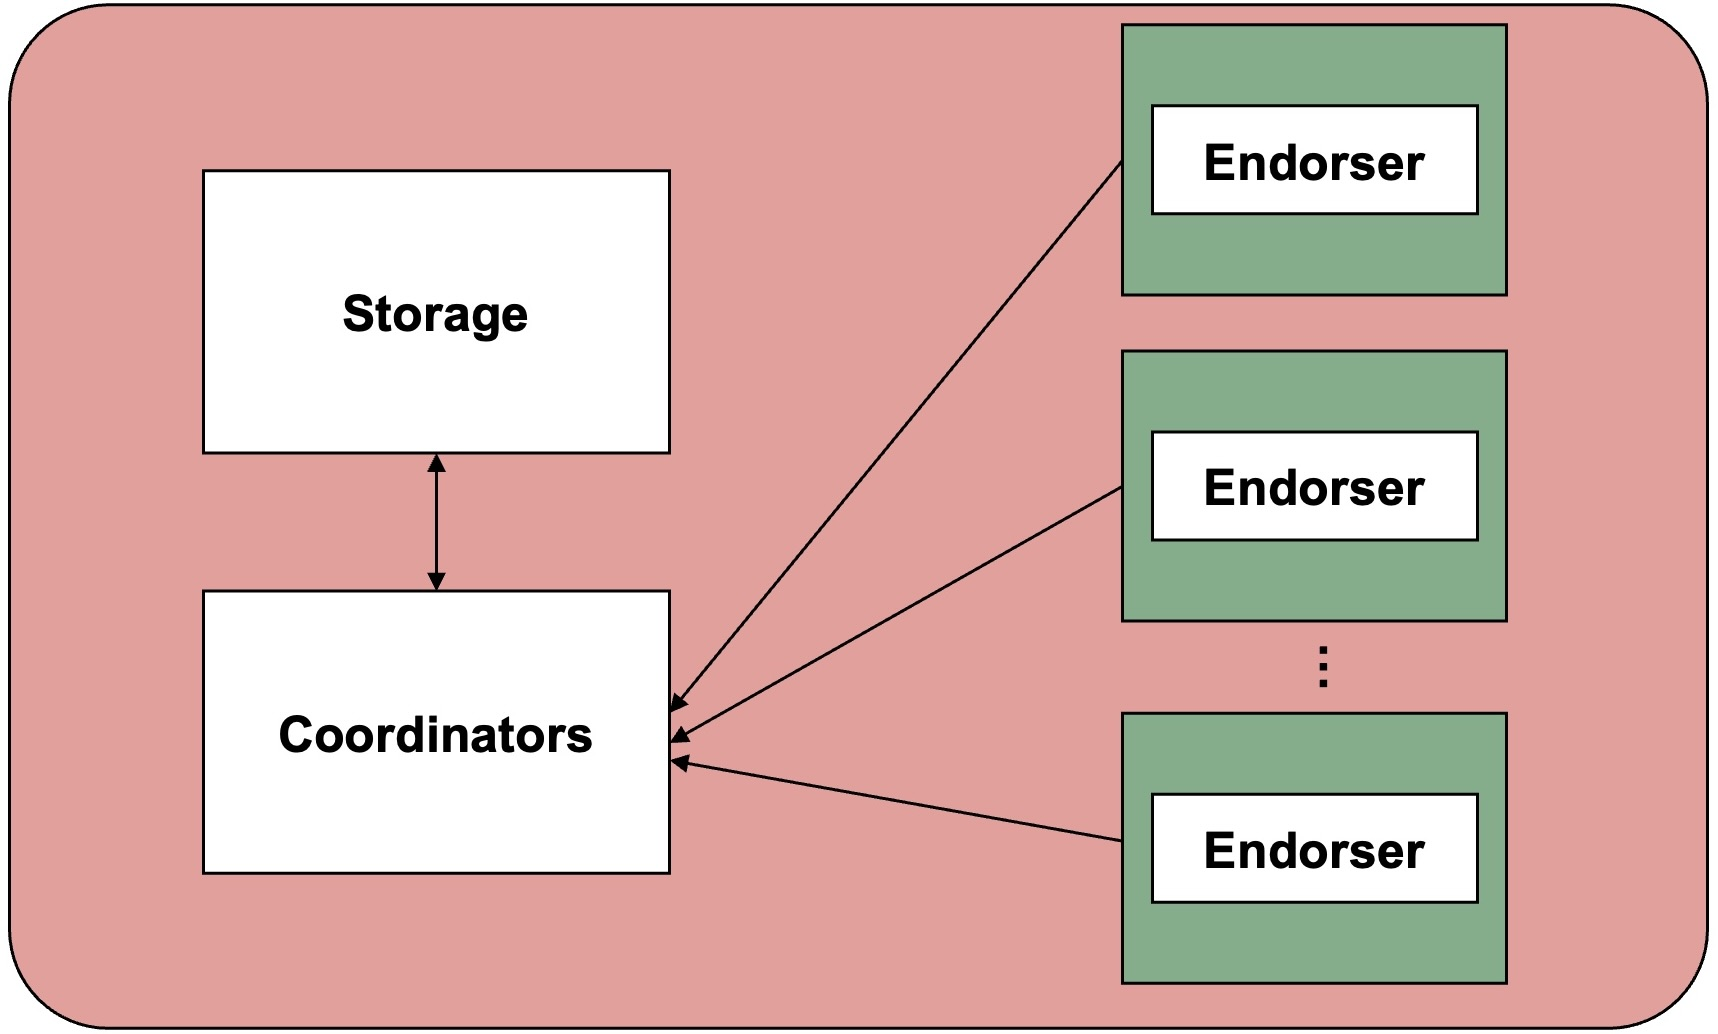
\includegraphics[scale=0.12]{pictures/nimble}
	\caption{Each node consists of a TEE. Inside the TEE there is the Endorser that saves the tail of the ledger.}
	\label{nimble}
\end{figure}

